\chapter{Execute Stage}

\section{Execute}

In the last lab, you created the ALU and ALU Control modules.  Now we will finish the iExecute stage.  The iExecute stage is represented by the red box in Figure ~\ref{fig:execute_stage}.  To finish the iExecute stage, you will need to add the following:
 
\begin{enumerate}
	\item Mux to select the source of the second input into the ALU.  You can reuse your mux that you created in the iFetch stage.
	\item Shifter to left shift the sign extended branch address offset.  You will need to create a new module for this.
	\item Adder to add the branch address offset to the current PC.  You can reuse your adder that you created in the iFetch stage.
\end{enumerate} 

\begin{figure}
	\caption{Execute Stage}\label{fig:execute_stage}
	\begin{center}
		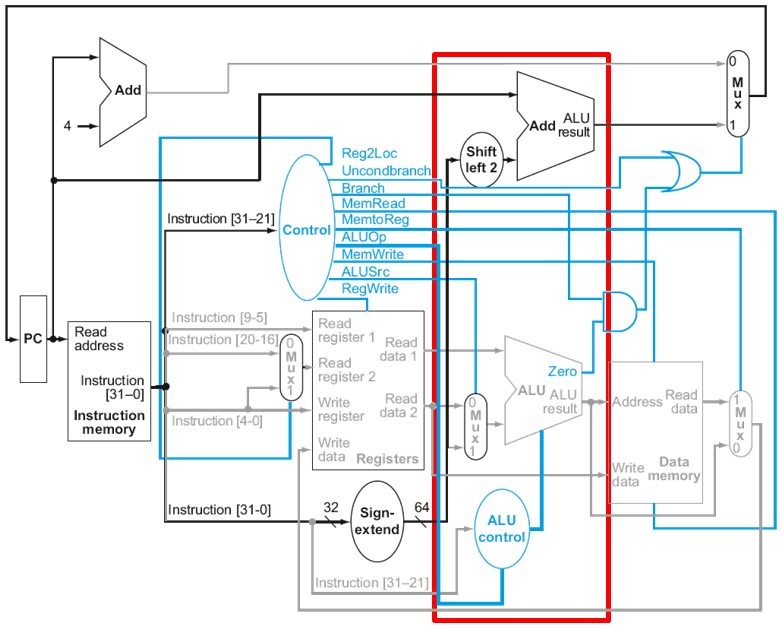
\includegraphics[width=4.75in]{../images/execute_stage.png}
	\end{center}
\end{figure} 

These five modules should be included in a new module called iExecute.  iExecute should consist of everything shown in the red box on Figure ~\ref{fig:execute_stage}. 

Next, create a test bench to verify that your iExecute module works correctly.  Use the 10 instructions from your Expected Results Table.  To do this successfully, you will need to evaluate which signals are inputs to the iExecute stage and provide the input values based on your previous Expected Results Table.  For example, the ALU Control module needs an input of opcode, so you would retrieve your opcode for each instruction from the opcode row of the Expected Results Table.  The iExecute module does not need a clock.  In addition to the inputs from your Expected Results Table, you will also need to provide a PC value.  In your test bench, this PC value should start at 0 and increment by 4 for each instruction.

\section{Your Assignment}
You are to:
\begin{enumerate}
\item Complete the iExecute module 
\item Update your Expected Results Table with the outputs from the iExecute stage.  Also add a PC value. 
\item Create an iExecute\_test module
\item Verify that your simulation results match your expected results.
\item Create a lab report in the LabN format.
\end{enumerate} 